This section analyzes the performance of \TF and compares it with \MNB by addressing the two research questions in Section~\ref{sec:EXP1} and Section~\ref{sec:EXP3}, respectively.

%discusses the findings of the qualitative assessment. To address the formulated research questions, we perform two different experiments. Section \ref{sec:EXP1} discusses the \TF results by variating different parameters. % We measure the predict performances of the \MNB in Section \ref{sec:EXP2}. 
%The results obtained with the entangled approach (\ie the combination of \TF and \MNB approaches) are investigate in Section~\ref{sec:EXP3} . 


\subsection{\rqfirst} \label{sec:EXP1}
  
To find the configuration obtaining the best prediction performances, we experimented %with different \TF configurations 
by varying the available parameters, \ie the number of neighbors \emph{k}, the number of recommended items \emph{N}. %, and the involved dataset.   %The former refers to the number of similar repositories used in the recommendation engine. 
%The latter value \emph{t} is used to select the input topics based on their frequencies: given an initial set of topics, we filter them with the cut-off value to reduce the noise in the original dataset. Then, the recommendation phase is enabled by varying the number of presented parameters. According to Section \ref{sec:methodology-metric}, N is the cut-off value and \emph{k} is the number of neighbours of the graph. We evaluate different configuration by setting N=1,5,10,15,20 and k=5,10,15,20,25. 
%Figure \ref{fig:configs} shows the results  in terms of precision and recall. 
%As we rely on a collaborative filtering technique, the number of output topics, the number of neighbors, and the data preprocessing play an important role in the assessment. 
To be more concrete, we chose two different values of \emph{N}, \ie \emph{N} = $\{5, 10\}$, and five values of \emph{k}, \ie \emph{k} = $\{5, 10, 15, 20, 25\}$. Furthermore, we also considered all the five datasets defined in Section~\ref{sec:Dataset}, \ie $D_{1}$, $D_{5}$, $D_{10}$, $D_{15}$, and $D_{20}$. The average success rates obtained by running the ten-fold cross-validation technique with \TFa are depicted in Fig.~\ref{fig:success-rateN5} and Fig.~\ref{fig:success-rateN10}.

%we use different topic frequency cut-off \emph{t} to remove very infrequent topics from the dataset. 
%The bar charts in Fig.~\ref{fig:success-rateN5} and \ref{fig:success-rateN10} show the average success rates obtained by running the ten-fold cross-validation technique with \TFa. %divided by the different topic frequency cut-off \emph{t}

%Both figures depict the results of \TF applied on the different datasets defined in Section~\ref{sec:Dataset}, \ie $D_{1}$, $D_{5}$, $D_{10}$, $D_{15}$, and $D_{20}$.
%In particular, Fig.~\ref{fig:success-rateN5} and Fig.~\ref{fig:success-rateN10} shows the success rate considering the first 5 and 10 recommended topics respectively. The horizontal axes shows the success rate outcomes for different size of neighbours \emph{N}.

Overall, it is evident that infrequent topics negatively affect the prediction outcomes. With $D_{1}$, \ie all projects are considered, \TF obtains a low success rate by both configurations N=5 and N=10, compared to the results of other cut-off values \emph{t}. For instance, with k=5, \TFa gets 0.54 as success rate for $D_{1}$, meanwhile it gets 0.62 as success rate for $D_{5}$ and $D_{10}$, and 0.63 for $D_{15}$ and $D_{20}$. The same trend can also be witnessed with other values of k, \ie \emph{k} = $\{10, 15, 20, 25\}$: \TFa achieves a better performance when we consider a dataset with more topics for each project. This is understandable since \TFa relies on the availability of training data to function: the more topics it has, the better it can compute the similarities among projects (cf. Fig.~\ref{fig:Graph} and Eq.~\ref{eqn:VsmSim}), and thus it is able to find more relevant topics (cf. Eq.~\ref{eqn:Prediction}). Similarly, for N=10, \ie we consider a longer list of recommendations, \TFa obtains a better success rate when a dataset with more detailed training data is exploited. 

\begin{figure*}[t]
\centering
	\begin{tabular}{c c}	
	\subfigure[N=5]{\label{fig:success-rateN5}
	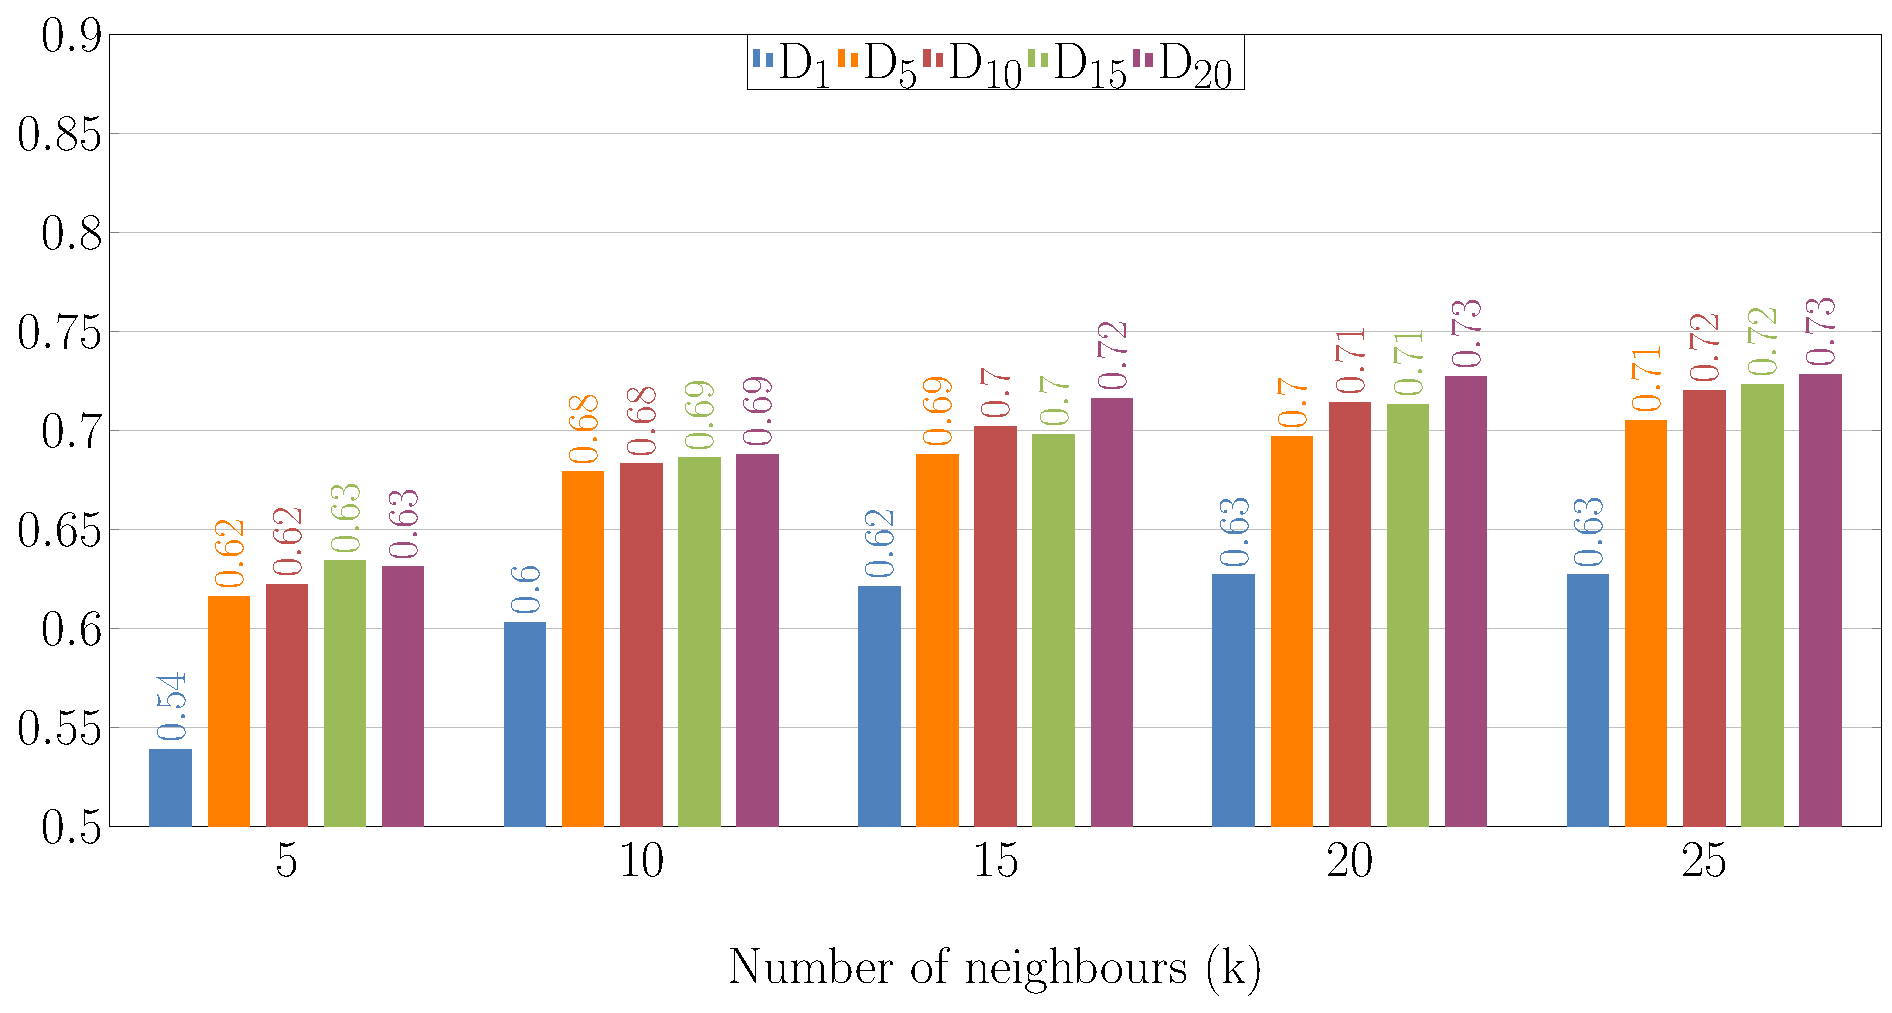
\includegraphics[width=0.48\linewidth]{figs/successRateN@5.pdf}} &
	\subfigure[N=10]{\label{fig:success-rateN10}
	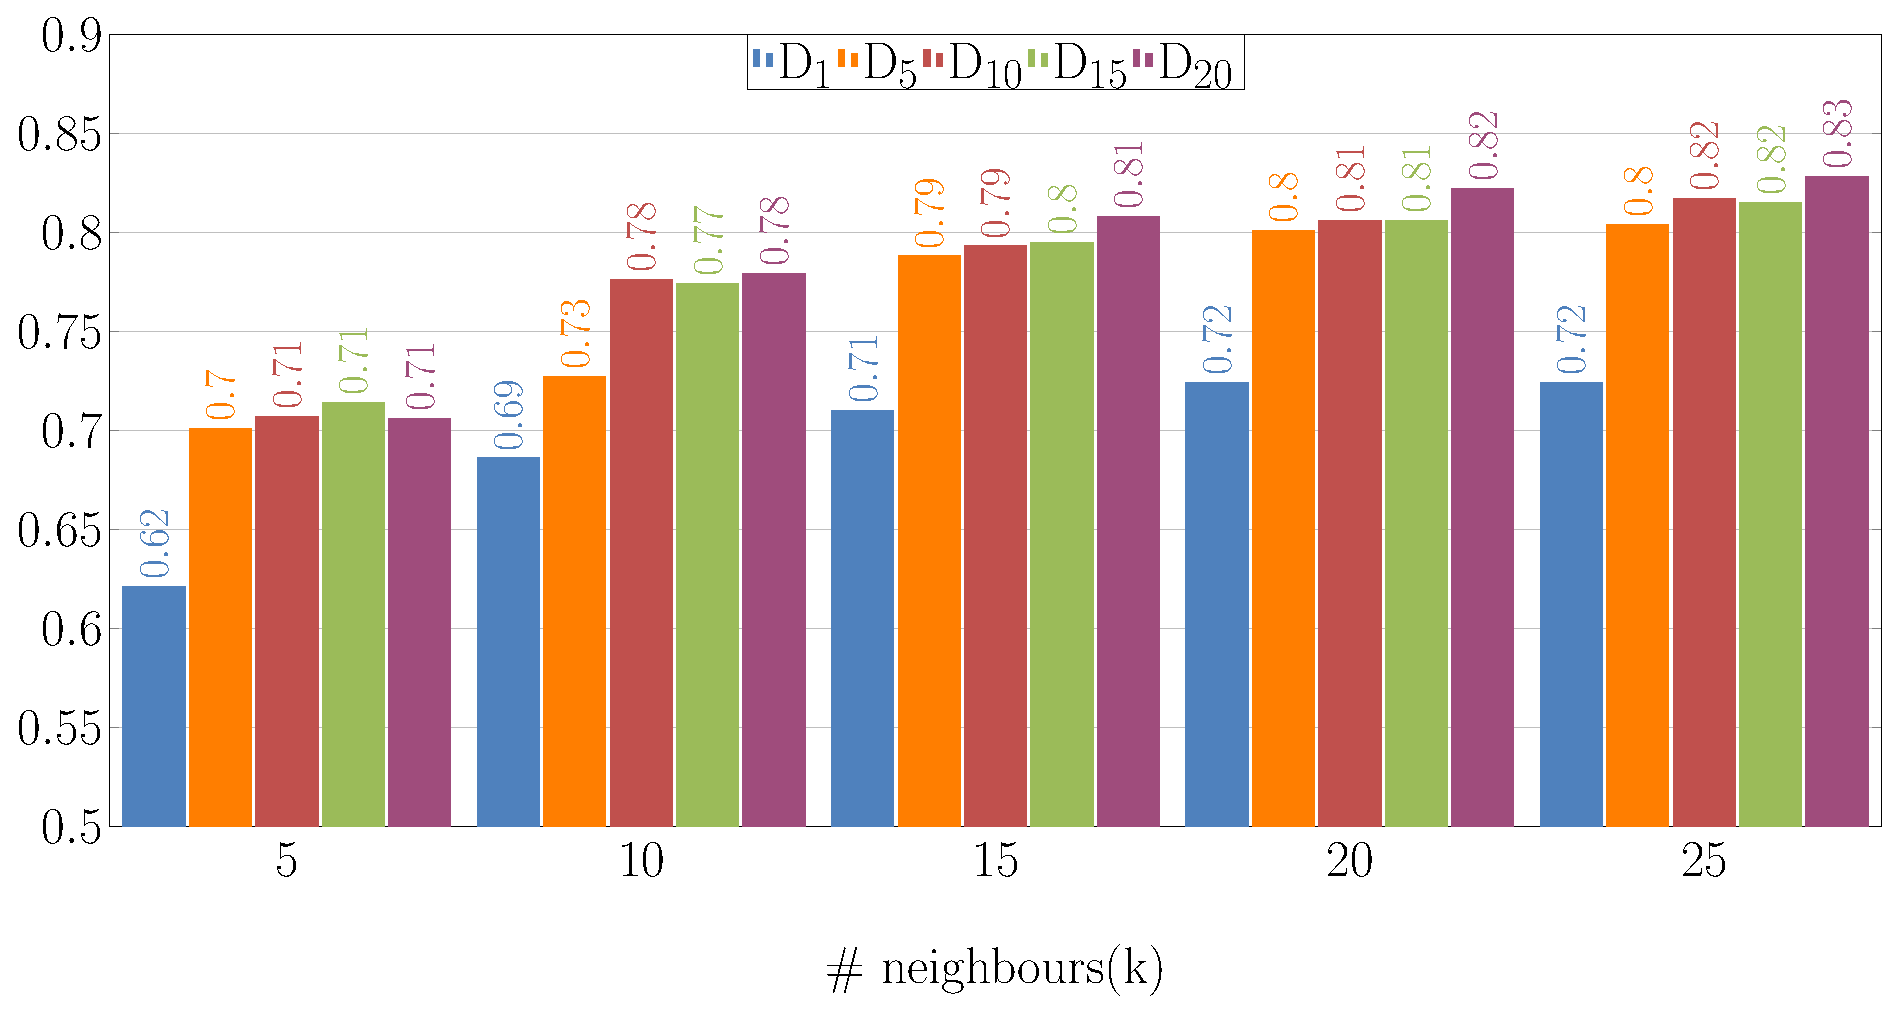
\includegraphics[width=0.48\linewidth]{figs/successRateN@10.pdf}}	
	\end{tabular} 
	\caption{Success rate with 5 and 10 input topics.}
	\label{fig:success5_10}
\end{figure*}
\begin{figure}[t!]
	\centering
	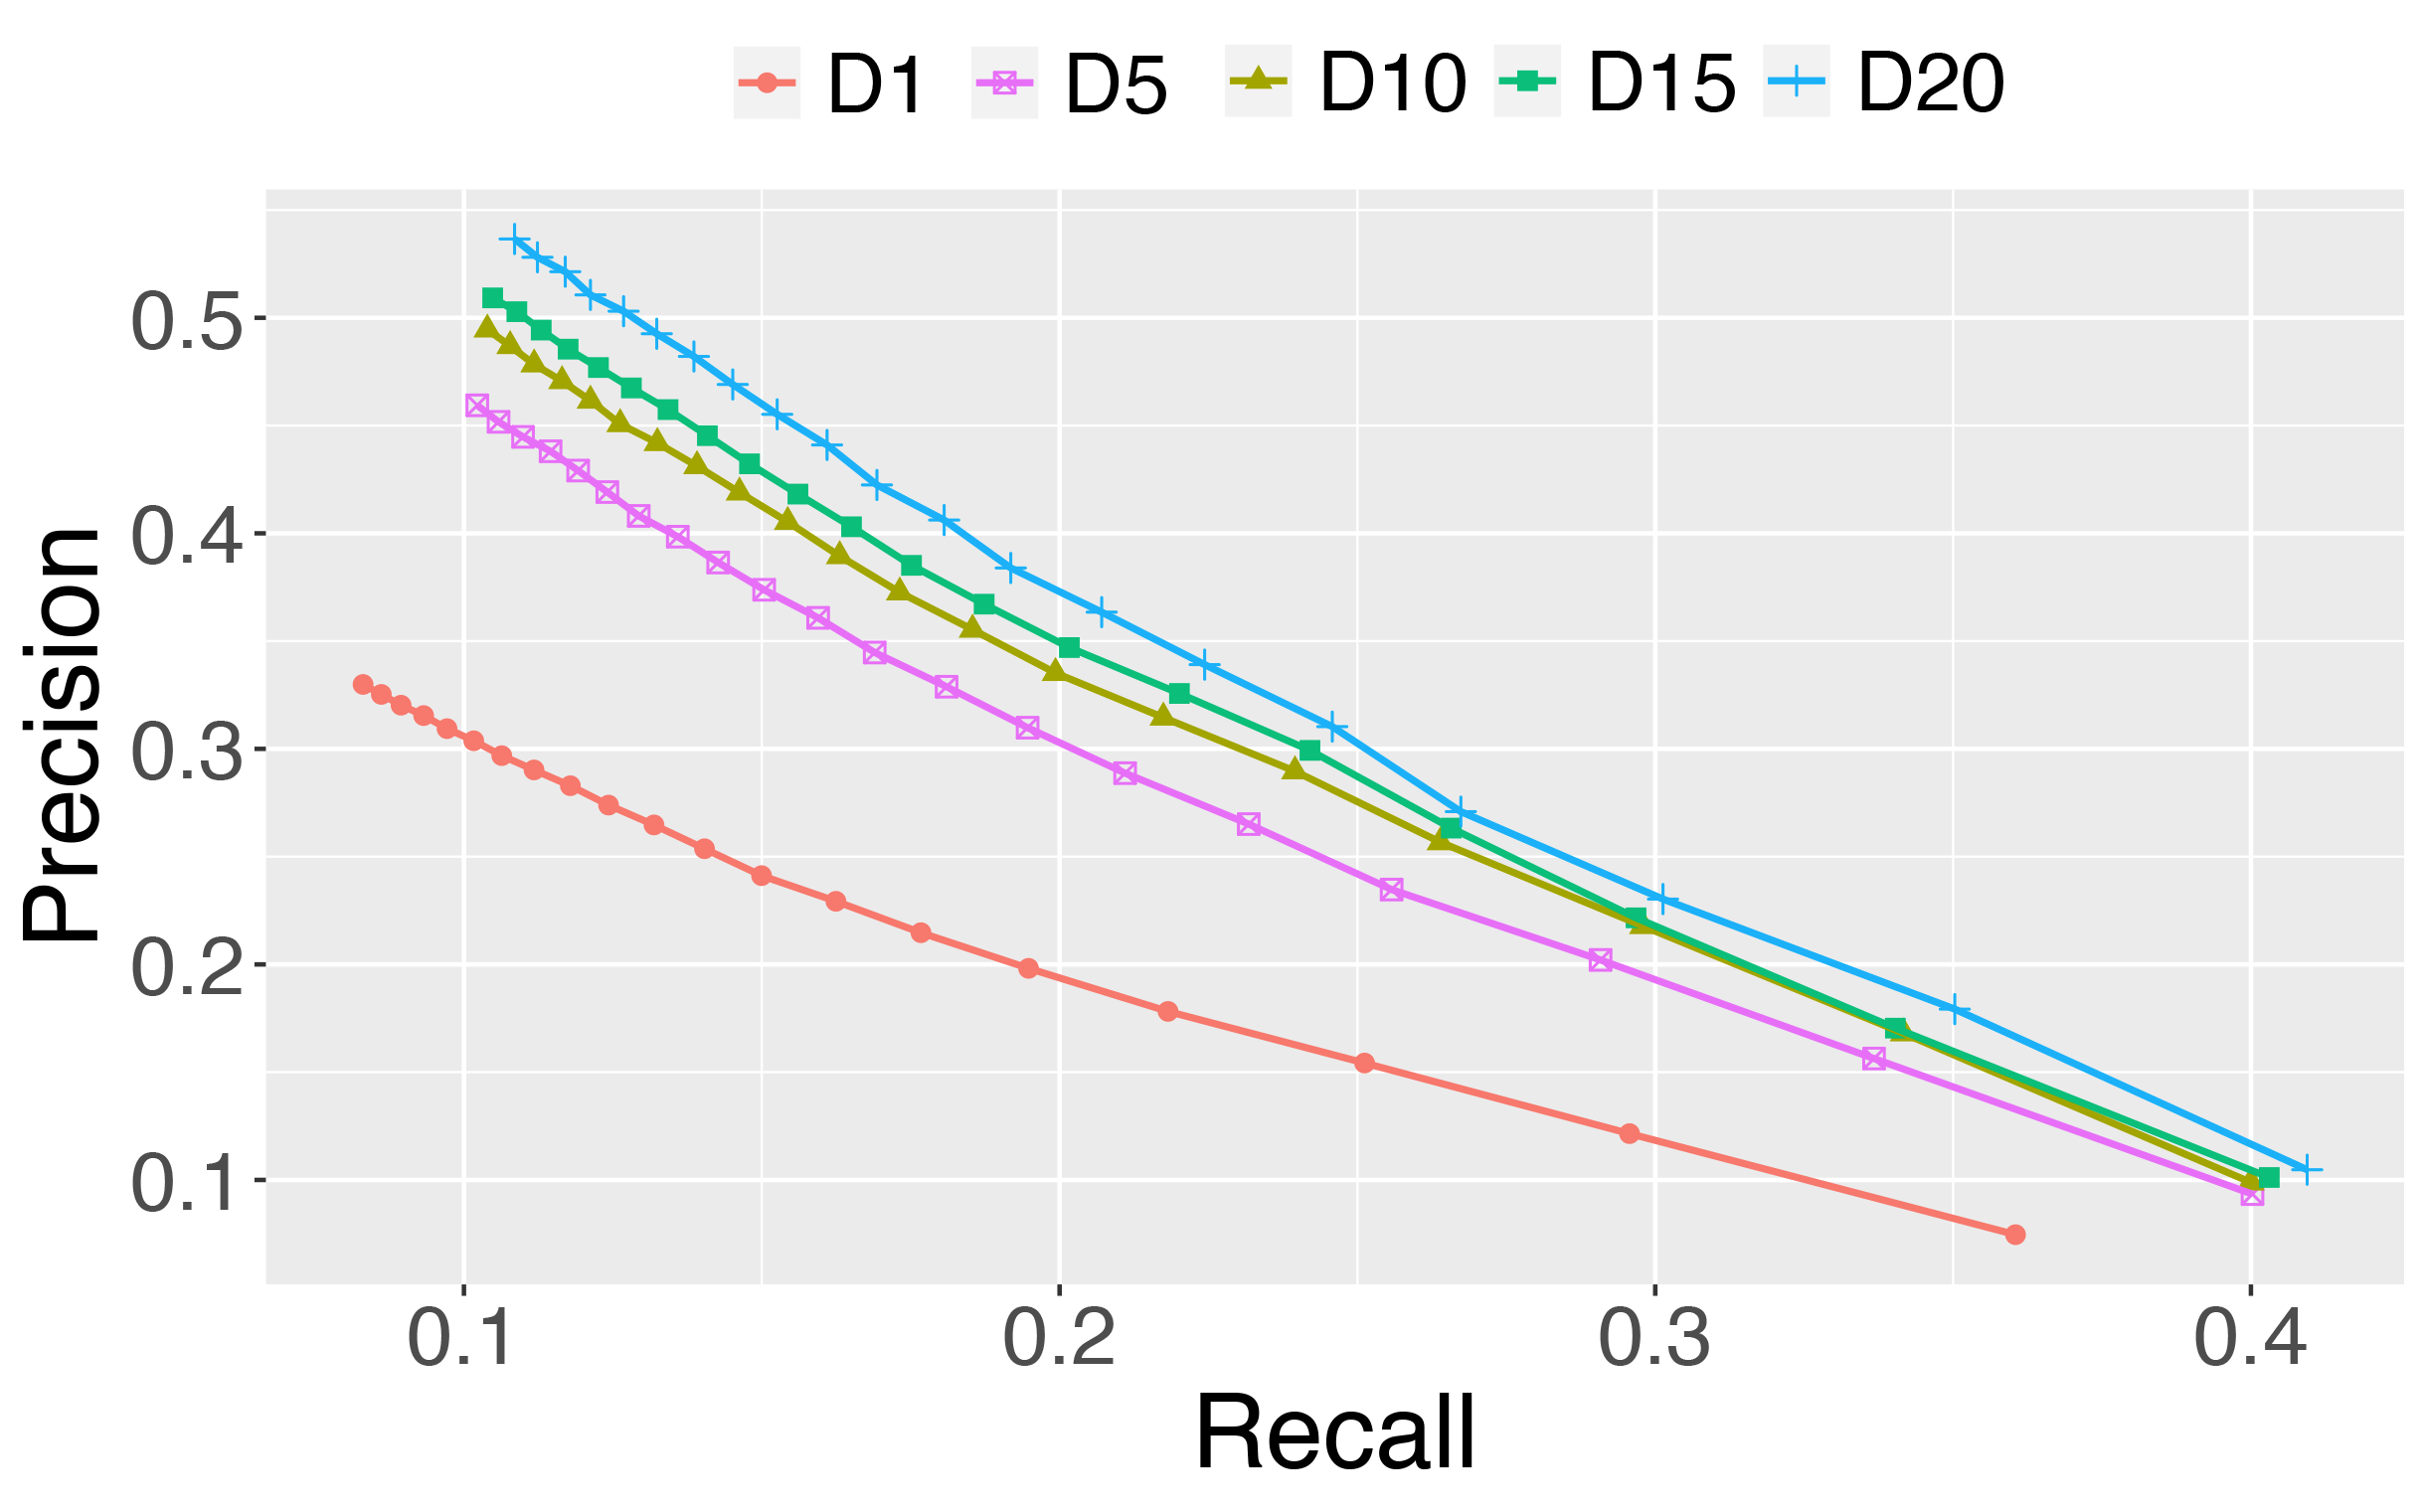
\includegraphics[width=0.80\linewidth]{figs/PrecisionRecallCurve.png}
	\caption{Precision/recall curves.}%Evaluation of the different configuration.
	\label{fig:configs}
\end{figure}

Next, we examine the influence of the number of neighbors k on the prediction performance. For N=5, from Fig.~\ref{fig:success-rateN5} it is clear that incorporating more neighbor projects for recommendation helps improve the performance considerably. Take as an example, for k=10 the best success rate is 0.69 obtained for $D_{20}$, and the corresponding score achieved with k=25 is 0.73 for $D_{20}$. For N=10, we see a clear gain in performance when more neighbors are considered for the computation of recommendations. The best obtained success rate is 0.83 when k=25 for $D_{20}$. As a whole, we come to the conclusion that increasing the number of neighbors used for computing missing ratings in the project-topic matrix is beneficial to the final recommendations. On the other hand, this also increases the computational complexity as comprehended in Eq.~\ref{eqn:Prediction}. Therefore, it is necessary to maintain a trade-off between accuracy and efficiency when deploying \TF by choosing a suitable value of k. 

%The success rate assessment exhibits an average improvement of 10\% in all of the possible configurations obtained by variating \emph{N} and \emph{k} values. In particular, the success rate archives better results by setting higher values of \emph{k}. Nevertheless, increasing the number of neighbours gives remarkable benefits only until a certain threshold. Given \emph{k} = 5, the success rate@5 passes from 63\% to 69\% if we consider k=10. This positive delta decreases by augmenting the number of neighbours until it reaches a stable success rate. Thus, we can consider \emph{k} = 25 as the maximum value capable of improving prediction performances. This trend is further confirmed by introducing more topics in the initial set. We also demonstrate that the topic filtering preprocessing fosters this enhancement and noise removal is a critical step of the entire process.


%This is also confirmed by the precision and recall curves depicted in

To further study \TF's performance, we computed and depicted in Fig.~\ref{fig:configs} the precision/recall curves (PRCs) for all the considered datasets. 
%From the accuracy scores computed using Eq. (5) and Eq. (6), the Precision-Recall curves (PRCs) for all 10 rounds of validation and different values of k were sketched. 
%The line graph depicts the precision and recall curves on average for all 10 rounds by considering 
For this setting, the number of recommended items \emph{N} was varied from 1 to 20, aiming to study the performance for a long recommendation list. Each dot in a curve corresponds to precision and recall obtained for a specific value of \emph{N}. Furthermore, we fixed k=25 since this number of neighbors brings the best prediction outcomes among others, while it still maintains a reasonable execution time. As a PRC close to the upper right corner represents a better precision/call~\cite{NGUYEN2020110460}, Fig.~\ref{fig:configs} demonstrates that by considering a dataset with more topics for each repository, \TFa yields a better prediction performance. In particular, the worst precision/recall relationship is seen by $D_{1}$, while the best one is obtained by $D_{20}$. Overall, these results are consistent with those presented in Fig.~\ref{fig:success-rateN5} and Fig.~\ref{fig:success-rateN10}: using projects consisting of more input topics helps \TFa enhance its performance substantially.

% an10 .
%These outcomes have been obtained by keeping 25 as the number of neighbours \emph{k} because we have already discussed that higher values of neighbours reach better prediction performances.
%Overall, the precision and recall values rise when the \emph{t} cut-off grows. Given that better prediction performance appears near to the upper right corner, the figure shows that a higher value of \emph{t} reaches better accuracy for all values of \emph{N}.

%~\cite{DiNoia:2012:LOD:2362499.2362501}

%As defined in Section~\ref{sec:metrics}, 

We investigate if \TFa can recommend a wide range of topics to repositories by considering catalog coverage. The metric measures the percentage of recommended topic in the training data that the model is able to suggest to a test set, and a higher value corresponds to a better coverage. 
%In our experiment, we measured the metric among topics, \ie 15,743. 
Table~\ref{tab:coverage} reports the average coverage value for the considered datasets, \ie $D_{1}$, $D_{5}$, $D_{10}$, $D_{15}$, $D_{20}$. %all ten rounds. 

%The average catalog coverage of all folds decreases from 9.306\% (Dt$_1$) to 1.805\% (Dt$_{20}$) because there are no training data to recommend infrequent topics. 
%The catalog coverage decreases because there are no training data to recommend infrequent topics. In particular, the average \emph{Global coverage} values decrease from 9.306\% (Dt$_1$) to 1.805\% (Dt$_{20}$).

From the table, we see that by considering a longer list of items, \ie increasing N, a better coverage is gained. Furthermore, using a higher cut-off value \emph{t} has a negative impacts on the global catalog coverage. For instance, with $D_{1}$ and N=2, we obtain 2.313 as coverage, and this score gradually decreases along \emph{t}, and shrinks to 0.715 with $D_{20}$. Similarly, by other values of N, catalog coverage is large for a low \emph{t} and small for a high \emph{t}. This can be explained as follows: setting a high value of \emph{t} means that a large amount of training data is discarded, and thus removing also topics. Altogether, we see that using a denser dataset for training, \ie projects with more topics, is beneficial to success rate, accuracy, but not to catalog coverage.

%Differently from the discussed metric outcomes, this experiment shows how an higher values of topic frequency cut-off negatively impacts on the catalog coverage metric.

As presented in Section~\ref{sec:methodology-metric}, given a testing project \emph{p}, a certain number of topics is used as input, \ie $\tau$, and the remaining ones are saved as ground truth data, \ie \emph{GT(p)}. We are interested to understanding how $\tau$ impacts on the prediction performance by performing a cross validation with $\tau$=$\{1,2,3,4,5\}$; Moreover, to simplify the evaluation, we fixed the number neighbors \emph{k} to 25 and the number of topics \emph{t} to 20. Fig.~\ref{fig:pr-input-topics} reports the average success rate obtained for two values of N, \ie N=$\{5,10\}$. %through our experiment. %ten folds by choosing different number of input topics. 
%Varying $\tau$ means changing the length of input topics that enable the \TF collaborative filtering recommender. 
%In this picture we report the average success of all folds values with \emph{k} = 25 and \emph{t} = 20 as configuration settings. 
The figure demonstrates an evident outcome: by using more input topics as input data, we get a better prediction performance. Take as an example, for $\tau$=1, we get a success rate of 0.44 and 0.61 for N=5 and N=10, respectively. When we use 5 topics to feed \TFa, the corresponding success rate is 0.56 and 0.66 for N=5 and N=10, respectively. This happens due to the fact that by considering more input topics, \TFa is able to better determine the similarity between the testing project and projects in the training data, as shown in Eq.~\ref{eqn:Prediction}, which eventually allows it to mine more relevant topics.

%The success rate values exhibits an improvements when the size of input topic rises. This behaviour demonstrate that \TF computes better similar repositories as neighbours when it has a higher number of topic as input. This is due to the similarity function that has been involved in the computation of first  \emph{k} neighbours. Because the average number of topics for each considered repository is 9.896 we can consider |\emph{t$_{in}$}| = 5 as the maximum value capable of improving prediction performances.
\begin{figure}[t!]
	\centering
	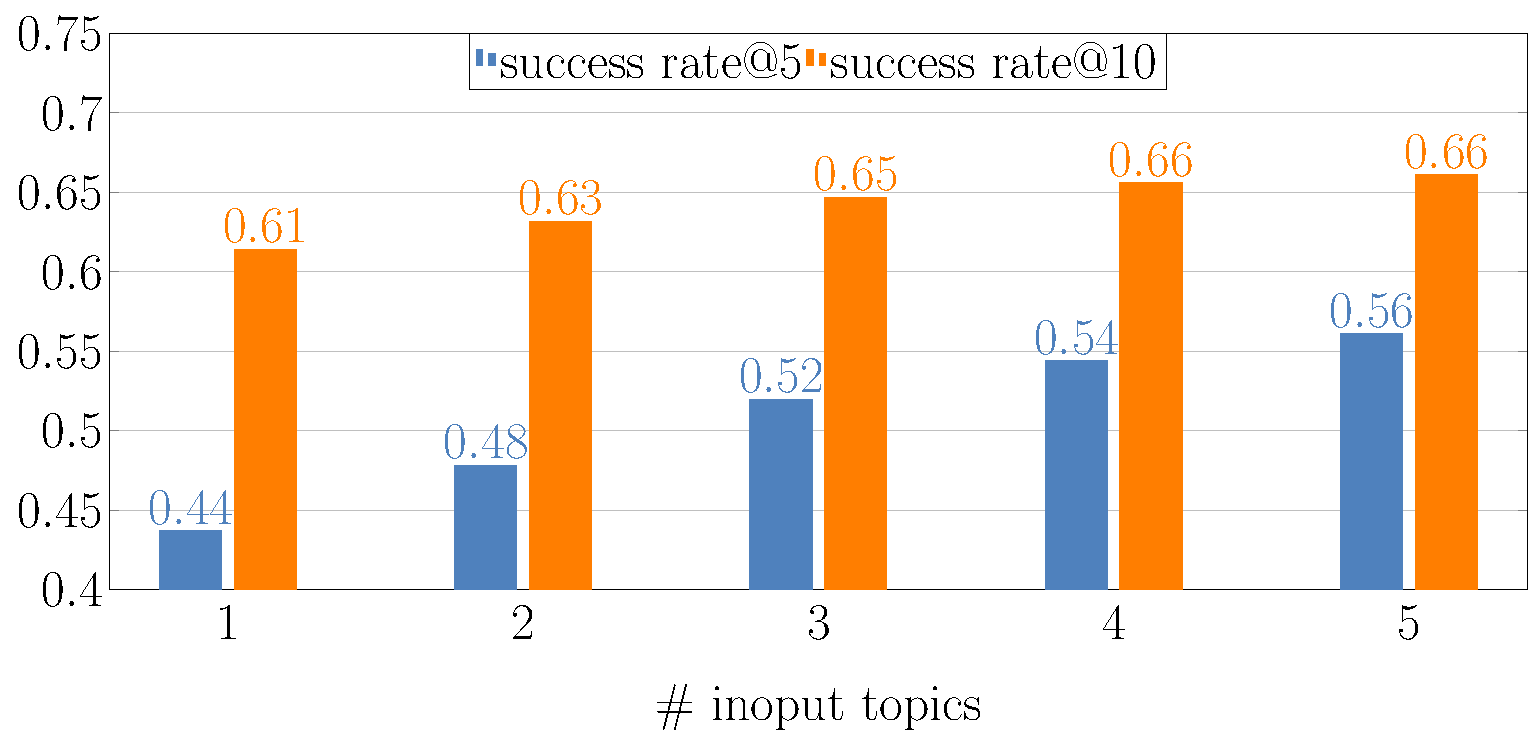
\includegraphics[width=0.8\linewidth]{figs/successRate_inputTopic.pdf}
	\caption{Success rates for $\tau$=$\{1,2,3,4,5\}$.}
	\label{fig:pr-input-topics}
\end{figure} 

%\begin{table*}[t]
%	\small
%\begin{tabular}{|l|p{1.2cm}p{1.2cm}|p{1.2cm}p{1.2cm}|p{1.2cm}p{1.2cm}|p{1.2cm}p{1.2cm}|p{1.2cm}p{1.2cm}|} \hline
%& \multicolumn{2}{c|}{Dt$_{1}$}                                                                                  & \multicolumn{2}{c|}{Dt$_{5}$}                                       & \multicolumn{2}{c|}{Dt$_{10}$}                                       & \multicolumn{2}{c|}{Dt$_{15}$}                                        & \multicolumn{2}{c|}{Dt$_{20}$}                                        \\ \hline
%
%\textbf{$N$}       & \textbf{Dataset coverage} & \textbf{Global coverage} & \textbf{Dataset coverage} & \textbf{Global coverage} & \textbf{Dataset coverage} & \textbf{Global coverage} & \textbf{Dataset coverage} & \textbf{Global coverage} & \textbf{Dataset coverage} & \textbf{Global coverage} \\ \hline
%2                & 2,313                       & 2,313                           & 11,339                      & 1,433                           & 17,558                       & 1,075                            & 21,991                       & 0,886                            & 24,220                       & 0,715                            \\ \hline
%4                & 3,925                       & 3,925                           & 18,698                      & 2,362                           & 28,634                       & 1,753                            & 35,766                       & 1,440                            & 38,681                       & 1,143                            \\ \hline
%6                & 5,494                       & 5,494                           & 25,583                      & 3,232                           & 38,317                       & 2,346                            & 46,130                       & 1,858                            & 50,044                       & 1,478                            \\ \hline
%8                & 7,075                       & 7,075                           & 31,940                      & 4,035                           & 46,296                       & 2,835                            & 54,265                       & 2,185                            & 58,791                       & 1,737                            \\ \hline
%10               & 8,720                       & 8,720                           & 37,899                      & 4,788                           & 52,904                       & 3,239                            & 61,027                       & 2,458                            & 65,011                       & 1,920                            \\ \hline
%12               & 10,385                      & 10,385                          & 43,314                      & 5,472                           & 59,044                       & 3,615                            & 67,093                       & 2,702                            & 70,484                       & 2,082                            \\ \hline
%14               & 12,073                      & 12,073                          & 48,436                      & 6,120                           & 64,249                       & 3,934                            & 72,385                       & 2,915                            & 75,275                       & 2,223                            \\ \hline
%16               & 13,872                      & 13,872                          & 53,261                      & 6,729                           & 68,852                       & 4,216                            & 76,682                       & 3,088                            & 79,187                       & 2,339                            \\ \hline
%18               & 15,753                      & 15,753                          & 57,402                      & 7,252                           & 73,080                       & 4,475                            & 80,553                       & 3,244                            & 82,659                       & 2,442                            \\ \hline
%20               & 17,746                      & 17,746                          & 61,497                      & 7,770                           & 76,738                       & 4,699                            & 83,649                       & 3,369                            & 85,363                       & 2,521                            \\ \hline
%\textbf{AVG} & \textbf{9,306}               & \textbf{9,306}                  & \textbf{37,495}              & \textbf{4,737}                  & \textbf{50,807}               & \textbf{3,111}                   & \textbf{58,089}               & \textbf{2,339}                   & \textbf{61,093}               & \textbf{1,805}                  \\ \hline
%\end{tabular}
%\caption{Coverage values for the proposed datasets (\ie D$_{1}$, D$_{5}$, D$_{10}$, D$_{15}$, D$_{20}$)}
%\label{tab:coverage}
%\end{table*}

\begin{table}[]
	\small
	\begin{tabular}{|l|l|l|l|l|l|}
		\hline
%		\multicolumn{1}{|c|}{\multirow{2}{*}{\textbf{N}}}                 & \multicolumn{5}{c|}{\textbf{Catalog Coverage}}                                                                                                                                                                                                                                                                                                                                          \\ \cline{2-6}
		
\textbf{N} & \textbf{ D$_{1}$} & \textbf{D$_{5}$} & \textbf{ D$_{10}$} & \textbf{D$_{15}$} & \textbf{D$_{20}$} \\ \hline
		2                & 2.313                                                                    & 1.433                                                                    & 1.075                                                                     & 0.886                                                                     & 0.715                                                                     \\ \hline
		4                & 3.925                                                                    & 2.362                                                                    & 1.753                                                                     & 1.440                                                                     & 1.143                                                                     \\ \hline
		6                & 5.494                                                                    & 3.232                                                                    & 2.346                                                                     & 1.858                                                                     & 1.478                                                                     \\ \hline
		8                & 7.075                                                                    & 4.035                                                                    & 2.835                                                                     & 2.185                                                                     & 1.737                                                                     \\ \hline
		10               & 8.720                                                                    & 4.788                                                                    & 3.239                                                                     & 2.458                                                                     & 1.920                                                                     \\ \hline
		12               & 10.385                                                                   & 5.472                                                                    & 3.615                                                                     & 2.702                                                                     & 2.082                                                                     \\ \hline
		14               & 12.073                                                                   & 6.120                                                                    & 3.934                                                                     & 2.915                                                                     & 2.223                                                                     \\ \hline
		16               & 13.872                                                                   & 6.729                                                                    & 4.216                                                                     & 3.088                                                                     & 2.339                                                                     \\ \hline
		18               & 15.753                                                                   & 7.252                                                                    & 4.475                                                                     & 3.244                                                                     & 2.442                                                                     \\ \hline
		20               & 17.746                                                                   & 7.770                                                                    & 4.699                                                                     & 3.369                                                                     & 2.521                                                                     \\ \hline
		\textbf{AVG} & \textbf{9.306}                                                           & \textbf{4.737}                                                           & \textbf{3.111}                                                            & \textbf{2.339}                                                            & \textbf{1.805}                                                            \\ \hline
	\end{tabular}
	\caption{Coverage values for the proposed datasets (\ie D$_{1}$, D$_{5}$, D$_{10}$, D$_{15}$, D$_{20}$)}
	\label{tab:coverage}
\end{table}


%On the other hand, a higher cut-off value \emph{t} negatively impacts on the global catalog coverage. For this reason, \emph{t} should be careful selected during the filtering phase to obtain balanced results in term of accuracy, success rate, and global catalog coverage.

\begin{tcolorbox}[boxrule=0.86pt,left=0.3em, right=0.3em,top=0.1em, bottom=0.05em]
\textbf{Answer to RQ$_1$.} \TFa achieves a better success rate and accuracy 
when more similar projects are considered for recommendation.
%\emph{k} and filtered data \emph{t}. %The number of neighbors and the topic filters contribute to this improvement. 
A higher cut-off value \emph{t} negatively impacts on the coverage; and using more topics as input data helps \TF improve the performance.
%However, the precision and recall values are still low, suggesting that bias lives in the users topic.
\end{tcolorbox}


%\subsection{\MNB evaluation} \label{sec:EXP2}

\rqsecond

Due to the lack of a baseline, we investigate the prediction performances of the \MNB to compare its outcomes with \CT. Reversely from the original paper, we apply the \MNB and we compared the outcomes whit respect to all topics (includin non featured ones) leaving the underlying structure untouched. This is necessary to undertake a fair comparison with \CT. Table \ref{tab:compareMNB} shows the evaluation results in terms  of the three aforementioned metrics. 


%\begin{table}[h]
%\centering
%
%
%\resizebox{8.5cm}{!} {
%\begin{tabular}{|l|l|l|l|l|l|l|}
%\hline
%  & \multicolumn{3}{c|}{ \textbf{\MNB}}          & \multicolumn{3}{c|}{ \textbf{\CT}}        \\ \hline
%\textbf{No. of input} & \textbf{Success rate} &\textbf{ Precision} & \textbf{Recall} & \textbf{Success rate} &\textbf{ Precision} &\textbf{ Recall} \\ \hline
%2  &       0.220       &    0.117       &  0.031       &     0.554         &      0.350     &   0.179      \\ \hline
% 4 &     0.392         &    0.119       &     0.063   &       0.682       &       0.267    &   0.271     \\ \hline
%6 &    0.538          &      0.122	     &   0.096     &     0.754         &    0.224       &   0.339     \\ \hline
%8 &    0.648          &  0.119         &   0.125      &         0.803     &     0.192      &   0.384     \\ \hline
%10 &      0.711        &    0.112       &   0.147     &      0.828        &   0.169        &    0.422    \\ \hline
%12 &     0.765         &      0.112     &   0.177     &        0.851      &     0.153      &     0.455   \\ \hline
%14 &      0.815        &    0.119       &   0.220     &    0.863          &   0.139         &   0.482     \\ \hline
%16 &       0.853       &     0.112      &     0.258   &        0.879      &   0.127        &   0.503     \\ \hline
%18 &      0.874        &     0.122      &     0.290   &       0.886       &     0.117      &    0.521    \\ \hline
%20 &     0.891         &    0.121       &    0.320    &      0.892        &   0.117        &       0.537 \\ \hline
%\rowcolor{Gray}
%\textbf{Average values} &    \textbf{0.651}        &   \textbf{ 0.120}       &   \textbf{ 0.165 }  &     \textbf{ 0.785}        &  \textbf{ 0.194}        &     \textbf{ 0.397 } \\ \hline
%\end{tabular}
%}
%\caption{Comparison of the two approaches.}
%\label{tab:compareMNB}
%\end{table} 
% Please add the following required packages to your document preamble:
% \usepackage[table,xcdraw]{xcolor}
% If you use beamer only pass "xcolor=table" option, i.e. \documentclass[xcolor=table]{beamer}
\begin{table}[]
	\scriptsize
	\resizebox{8.5cm}{!} {
	\begin{tabular}{|l|l|l|l|l|l|l|}
		\hline
		\rowcolor[HTML]{C0C0C0} 
		& \multicolumn{2}{c}{\textbf{Success rate}}         & \multicolumn{2}{|c|}{\textbf{Precision}}            & \multicolumn{2}{c|}{\textbf{Recall}}               \\ \hline
	 \rowcolor[HTML]{C0C0C0} 
		\textbf{\emph{N} } & \textbf{MNB} & \textbf{\CT }& \textbf{MNB} & \textbf{\CT} & \textbf{MNB} & \textbf{\CT }\\ \hline
		2                       & 0.220               & 0.554              & 0.117               & 0.350              & 0.031               & 0.179              \\
		4                       & 0.392               & 0.682              & 0.119               & 0.267              & 0.063               & 0.271              \\
		6                       & 0.538               & 0.754              & 0.122               & 0.224              & 0.096               & 0.339              \\
		8                       & 0.648               & 0.803              & 0.119               & 0.192              & 0.125               & 0.384              \\
		10                      & 0.711               & 0.828              & 0.112               & 0.169              & 0.147               & 0.422              \\
		12                      & 0.765               & 0.851              & 0.112               & 0.153              & 0.177               & 0.455              \\
		14                      & 0.815               & 0.863              & 0.119               & 0.139              & 0.220               & 0.482              \\
		16                      & 0.853               & 0.879              & 0.112               & 0.127              & 0.258               & 0.503              \\
		18                      & 0.874               & 0.886              & 0.122               & 0.117              & 0.290               & 0.521              \\
		20                      & 0.891               & 0.892              & 0.121               & 0.117              & 0.320               & 0.537              \\ \hline
		\rowcolor[HTML]{C0C0C0} 
		\textbf{Average} & \textbf{0.651}      & \textbf{0.785}     & \textbf{0.120}      & \textbf{0.194}     & \textbf{0.165}      & \textbf{0.397}    \\ \hline
	\end{tabular}}
\caption{Comparison of the two approaches.}
\label{tab:compareMNB}
\end{table}
We evaluate both approaches by variating the number of recommended topics up to 20. For the sake of the presentation, we report half of the data as we aim to show the overall trend.
As we can see, \CT outperforms the \MNB considering all the metrics. In particular, the success rate grows according to the number of input for both of the approaches. Although the \MNB reaches the same values of \CT with 20 input topics, the latter starts from an initial success rate value of 55\%. This statement holds for all metrics considered in the comparison. A significant achievement is given by the recall value which is the almost triplicated on average using \CT as the recommendation engine. For some input, the \MNB slightly outperforms \CT even though they are meaningless compared to the other findings. 
This gap is explained by the \MNB model features. In this comparison, we have added the not featured topics to the possible set of outputs \footnote{Due to the space issues, we cannot explain in detail the \MNB internal construction. Thus, the interested reader can find more information in the related work}. Consequently, the accuracy of the model is compromised by these new possible outcomes that the \MNB is not able to provide. This impacts especially on the recall values, as proved by the experiment. The aim of this comparison is to prove the soundness of \CT as a recommendation algorithm where the possible outcomes are heterogeneous \ie featured topics are shuffled with not featured ones. However, the accuracy is very low compared with the success rate. This could be affected by the similarity function embedded in the recommendation engine. 


\begin{tcolorbox}[boxrule=0.86pt,left=0.3em, right=0.3em,top=0.1em, bottom=0.05em]
From the evaluation, we can claim that \CT outperforms the \MNB. This result is lead by the construction differences between the two approaches, even though the \MNB performances are negatively affected by the introduction of the not featured topics. This demonstrates the rightness of \CT in a miscellaneous environment. 
\end{tcolorbox}

\subsection{\rqsecond} \label{sec:EXP3}

As already reasoned in Section~\ref{sec:methodology-metric}, it is not feasible to directly compare \TF with \MNB, as they are based on different recommendation mechanisms. \TF relies on a supervised learning technique, requiring an initial set of assigned topics for the training. Meanwhile, \MNB works on the basis of an unsupervised learning system, which needs only data mined from README files to recommend, without being fed with any input topics.

In this research question, we aim to show that augmenting \MNB with \TF helps boost up the recommendation outcomes provided by \MNB. In particular, we run \TF on the outputs produced by \MNB, attempting to generate a more relevant list of items. %as input. %However, we can compare.

%Due to the internal construction of the \MNB, the direct comparison of the two approaches can bring biased results. Thus, we combined the two approaches to investigate potential improvements. We create this \emph{entagled} configuration by feeding \TF with the results of the \MNB. This simulates the exact use case of the collaborative filtering approach, in which the developer is represented by the \MNB. 

We conducted experiments on two of the selected datasets, \ie $D_{1}$ and $D_{20}$, as they correspond to two distinct levels of data completeness: $D_{1}$ has more projects but with a lower quality, while $D_{1}$ has fewer data but with a higher quality. In the experiment, $\tau$ was set to 5 since through RQ$_1$, we realized that this value fosters the best performance, among others. %With these two datasets, we aim at studying the performance of \TF in different . 
%lower and higher topic to be recommended respectively.
%Table \ref{tab:combined} summarizes the results of this experiment by comparing the \MNB and the entangled approach. From the previous assessment, we figured out that \TF reaches best results considering the Dataset $D_{20}$. Thus, we choose this one to conduct this second evaluation. 
%Furthermore, we varied the number of recommendation items as well as the number of input topics \ie \emph{N} and \emph{Tin} values respectively. From the previous assessment, we figured out that the number of inputs leading the best results is Tin=5. Thus, we compare the outcomes considering the minimum number of input topics provided by the \MNB, \ie Tin=2. 
The success rate, precision, recall and coverage scores obtained for $D_{1}$ and $D_{20}$ are reported in Table~\ref{tab:combined_dt1} and Table~\ref{tab:combined_dt20}, respectively. 

The results shown in Table~\ref{tab:combined_dt1} demonstrate that compared to \TF, \MNB obtains a better prediction performance in terms of success rate, recall and precision for a ranked list with a low number of items, \ie N $\leq$ 4. In particular, with N=2, \MNB gets 0.240 as success rate, while the corresponding score by \TF for 0.148. The same trend can be seen with recall and precision. This is understandable as \MNB relies on only README file(s) to function, and its performance is not affected by the number of considered topics. In contrast, \TF needs input topics to provide recommendation, that is the reason why for a dataset with a low quality dataset (with respect to the number of topics), \TF gets a moderate performance. %.the success rate achieved by \MNB is better than that of 

Table~\ref{tab:combined_dt1} also shows that \TF outperforms \MNB when we consider a longer list of recommended items. To be concrete, starting from N=6 (\ie the row marked with gray), all the metrics computed with \TF are superior to those computed with \MNB. For example, \TF gets 0.675 as the maximum success rate, while the corresponding score by \MNB is 0.662. More importantly, \TF always achieves a much better coverage than that of \MNB: By the best configuration, \TF reaches a coverage of 3.544, which is much higher than 0.768 obtained by \MNB. In other words, our proposed approach is able to recommend a wider range of topics than \MNB. This can be explained by the fact that \TF takes into consideration a set of topics as input, and the more data it has, the larger the set of topics it can recommend.

By examining Table~\ref{tab:combined_dt20}, we encounter a similar outcome compared to that of Table~\ref{tab:combined_dt1}: \TF outperforms \MNB by all the quality metrics, \ie success rate, recall, precision and coverage. Especially, using $D_{20}$ as the training data, \TF improves the overall success rate considerably, with respect to using $D_{1}$. This further confirms our findings in RQ$_1$: A denser dataset facilitates the capability of recommending a more relevant set of topics. %to repositories.

%The results demonstrate that the \MNB gains notable improvement by means of the entangled configuration in terms of the mentioned metrics \ie accuracy, success rate, and catalog coverage. We witness that \TF outperforms the \MNB by augmenting the number of recommended items. 
%The results in Table~\ref{tab:combined_dt20} demonstrate that the \MNB gains notable improvement by means of the entangled configuration in terms of the mentioned metrics \ie accuracy, success rate, and catalog coverage.
%Table~\ref{tab:combined_dt1} also confirms this trend by performing the same experiment with \emph{D$_1$} dataset. We witness that \TF outperforms the \MNB by augmenting the number of recommended items. For both datasets \ie \emph{D$_1$} and \emph{D$_{20}$}, after K=8 the accuracy and success rate overcomes the \MNB results considering the \TF's best configuration even though the overall accuracy trend is decreasing. This happens because enlarging the set of recommended items impacts negatively on the precision values. Reversely, the success rate rises up to 0.855 and 0.531 with \emph{D$_1$} and \emph{D$_{20}$} respectively. As witnessed for the accuracy value, the \MNB records better results until a certain threshold of output items. This degradation in performance is due to the internal probabilistic model used by the approach. 

% Please add the following required packages to your document preamble:
% \usepackage{multirow}
\begin{table*}[t!]
	\normalsize
	\small
\caption{Comparison between \MNB and \textit{MNBN+\TFb} using Dataset $D_{1}$.} 
%Experimental results obtained by
	\vspace{-.3cm}
\begin{tabular}{|c| c|c| c|c |c|c |c|c|} \hline
	& \multicolumn{2}{c|}{\textbf{Success rate}} & \multicolumn{2}{c|}{\textbf{Recall}} & \multicolumn{2}{c|}{\textbf{Precision}} & \multicolumn{2}{c|}{ \textbf{Catalog coverage}} \\ \hline
	$N$  & \MNB     & \textit{MNBN+\TFb}  & \MNB      & \textit{MNBN+\TFb}   & 
	\MNB       & \textit{MNBN+\TFb}    & \MNB       & \textit{MNBN+\TFb}      
	\\ \hline         
	
2        & 0.240    & 0.148  & 0.026    & 0.017   & 0.137    & 0.077     & 0.175   & 0.411   \\ \hline
4        & 0.383    & 0.287  & 0.042    & 0.035   & 0.123    & 0.081     & 0.314   & 0.617   \\ \hline
\rowcolor{Gray}
6        & 0.441    & 0.449  & 0.049    & 0.064   & 0.104    & 0.098     & 0.398   & 0.919   \\ \hline
8        & 0.499    & 0.531   & 0.055    & 0.085   & 0.093    & 0.098   & 0.474   & 1.272   \\ \hline
10       & 0.550    & 0.572   & 0.061    & 0.100   & 0.087    & 0.092   & 0.557   & 1.626   \\ \hline
12       & 0.584    & 0.603   & 0.066    & 0.111   & 0.081    & 0.086   & 0.620   & 2.008   \\ \hline
14       & 0.601    & 0.624   & 0.067    & 0.120   & 0.074    & 0.080   & 0.658   & 2.431   \\ \hline
16       & 0.616    & 0.643   & 0.068    & 0.128   & 0.067    & 0.074   & 0.687   & 2.825   \\ \hline
18       & 0.632    & 0.660   & 0.069    & 0.136   & 0.062    & 0.070   & 0.718   & 3.169   \\ \hline
20       & 0.662    & 0.675   & 0.073    & 0.143   & 0.060    & 0.066   & 0.768   & 3.544   \\ \hline
\end{tabular}
\label{tab:combined_dt1}
\end{table*}


\begin{table*}[t!]
	\normalsize
	\small
	\caption{Comparison between \MNB and \textit{MNBN+\TFb} using Dataset 
	$D_{20}$.}
	\vspace{-.3cm}
	\begin{tabular}{|c| c|c| c|c |c|c |c|c|} \hline		
		& \multicolumn{2}{c|}{\textbf{Success rate}} & \multicolumn{2}{c|}{\textbf{Recall}} & \multicolumn{2}{c|}{\textbf{Precision}} & \multicolumn{2}{c|}{ \textbf{Catalog coverage}} \\ \hline
		$N$  & \MNB     & \textit{MNBN+\TFb}  & \MNB      & 
		\textit{MNBN+\TFb}   & \MNB       & \textit{MNBN+\TFb}    & \MNB       
		& \textit{MNBN+\TFb}      \\ \hline         
		
		2  & 0.363      & 0.217  & 0.035     & 0.031  & 0.206       & 0.118   & 0.263          & 0.249      \\ \hline		
4  & 0.600      & 0.389  & 0.075     & 0.063  & 0.221       & 0.119   & 0.562         & 0.444     \\ \hline
6  & 0.635      & 0.601  & 0.094     & 0.121  & 0.187       & 0.153   & 0.715         & 0.612     \\ \hline 
\rowcolor{Gray}
8  & 0.680      & 0.704  & 0.106      & 0.171  & 0.159        & 0.162   & 0.810       & 0.848     \\ \hline
10 & 0.701      & 0.754  & 0.116      & 0.204  & 0.140        & 0.156   & 0.890       & 1.022  \\ \hline		
12 & 0.719      & 0.788  & 0.124      & 0.230  & 0.124        & 0.146   & 0.950       & 1.178     \\ \hline		
14 & 0.733      & 0.808  & 0.130      & 0.254  & 0.111        & 0.138   & 0.994       & 1.330     \\ \hline		
16 & 0.745      & 0.829  & 0.135      & 0.274  &  0.101       & 0.131   & 1.035       & 1.463     \\ \hline		
18 & 0.759      & 0.840  & 0.143      & 0.290  & 0.095        & 0.123   & 1.090       & 1.582     \\ \hline
20 & 0.772      & 0.855 & 0.150       & 0.306  & 0.090        & 0.117   & 1.148       & 1.701    \\ \hline
	\end{tabular}
	\vspace{.2cm}
	\label{tab:combined_dt20}
\end{table*}






%In particular, after Out=8 the accuracy and success rate overcomes the \MNB results considering the \TF's best configuration even though the overall accuracy trend is decreasing. This happens because enlarging the set of recommended items impacts negatively on the precision values. Reversely, the success rate rises up to 0.855 with the best configuration of the entangled approach. As witnessed for the accuracy value, the \MNB records better results until a certain threshold of output items. This degradation in performance is due to the internal probabilistic model used by the approach. 



%Table \ref{tab:combined_dt1} and~\ref{tab:combined_dt20}  summarize the results of this experiment by comparing the \MNB and the entangled approach for $D_1$ and $D_{20}$ respectively. 
%For experiment purposes, we variate the number of recommendation items as well as the number of input topics \ie \emph{N} and \emph{Tin} values respectively. From the previous assessment (see Figure~\ref{fig:pr-input-topics}), we figured out that the number of inputs leading the best success rate results is 5. Thus, we compare the outcomes considering the minimum number of input topics provided by the \MNB, \ie Tin=2. 


%\begin{table}[h]
%\centering
%
%
%\resizebox{8.5cm}{!} {
%\begin{tabular}{|l|l|l|l|l|l|l|}
%\hline
%  & \multicolumn{3}{c|}{\textbf{\TF}}          & \multicolumn{3}{c|}{\textbf{Entangled approach}}        \\ \hline
%\textbf{No. of input} & \textbf{Success rate} &\textbf{ Precision} & \textbf{Recall} & \textbf{Success rate} &\textbf{ Precision} & \textbf{Recall} \\ \hline
%1  &       0.409       &    0.409       &  0.105       &     0.138         &      0.221     &   0.029      \\ \hline
% 2 &     0.554         &    0.350       &     0.179   &       0.220       &       0.198    &   0.053     \\ \hline
%3 &    0.632          &      0.301	     &   0.230     &     0.304         &    0.192       &   0.077     \\ \hline
%4 &    0.682          &  0.267         &   0.271      &         0.393    &     0.186      &   0.099     \\ \hline
%5 &      0.728        &    0.246       &   0.310     &      0.479        &   0.183        &    0.122    \\ \hline
%\rowcolor{Gray}
%6 &     0.754         &      0.224     &   0.339     &        0.983      &     0.278      &     0.225   \\ \hline
%7 &      0.778        &    0.207       &   0.363     &    0.999          &   0.340         &   0.322     \\ \hline
%8 &       0.803       &     0.192      &     0.384   &        1      &   0.371        &   0.40     \\ \hline
%10 &      0.828        &     0.169      &     0.422   &       1       &     0.382      &    0.511    \\ \hline
%15 &     0.872         &    0.132       &    0.493    &      1        &   0.322       &       0.636 \\ \hline
%20 &     0.892         &    0.117       &    0.537    &      1        &   0.266        &       0.696 \\ \hline
%\rowcolor{Gray}
%\textbf{Average values} &    \textbf{ 0.785}        &   \textbf{ 0.194}       &   \textbf{ 0.397}   &     \textbf{ 0.826 }       &  \textbf{ 0.296}        &       \textbf{0.433}  \\ \hline
%\end{tabular}
%}
%\caption{Results for the entangled approach.}
%\label{tab:combined}
%\end{table} 

%Although the examined metrics are useful to analyze the overall performances, the catalog coverage can evaluate properly the capability to recommend a \emph{list} of items instead of a single one. Looking at the results, we can observe a substantial increase after 8 output items. As expected, the coverage dramatically increases with a larger number of outcomes for both of the considered approaches. Nevertheless, the positive gap of the entangled configuration is greater than the \MNB value. Considering the Out=20, the maximum value reached by the \MNB is 39.636 while the best configuration in the entangled experiment reaches a coverage of 58.725.
%These findings can be explained by considering the nature of the considered topics. As said before, the \MNB can predict only featured topics as training the entire set of \GH topics is not possible due to the computation issues. Reversely, \TF covers a larger set of topics by enabling the described collaborative filtering technique. In this way, the \emph{entangled} is capable of suggesting both featured and not featured topics to the final user and enlarging the possible set of outcomes.



\begin{tcolorbox}[boxrule=0.86pt,left=0.3em, right=0.3em,top=0.1em, bottom=0.05em]
\textbf{Answer to RQ$_2$.} Compared to \MNB, \TFb substantially improves the prediction performance with respect to success rate, precision and recall. Moreover, while \MNB suffers a low catalog coverage, \TFb is able to recommend a wide range of topics to repositories.
\end{tcolorbox}

%, as clearly demonstrated by the higher value of the entangled experiment
%By varying both the input and output number of topics, the accuracy and success rate experienced an enhancement even though the former reached low values. 









